\begin{frame}{Conditional Probability}
    We can get far more information out of the relationships between multiple variables than we can from a single variable.
    
    For example
    \begin{itemize}
        \item Recall our case study on the malaria vaccine.
        \item We can look at P(infection), but that doesn't tell us anything about the efficacy of the vaccine.
        \item Instead, we want to look at the probability that a person develops infection \textit{if they were vaccinated}.
        \item We compare this to the probability that a person develops infection if they were not vaccinated.
    \end{itemize}
\end{frame}

\begin{frame}{Contingency Table Probabilities}
    Let's consider a data set on a machine learning classifier. 
    \begin{itemize}
        \item The classifier is designed to take images and determine whether each one is about fashion.
        \item The classifier groups 1822 photos into either "fashion" or "not fashion".
        \item Separately, these photos are grouped into "fashion" and "not fashion" by a group of people.
        \begin{itemize}
            \item We take these groupings as the truth that the classifier is trying to get at.
        \end{itemize}
    \end{itemize}
\end{frame}

\begin{frame}{Contingency Table Probabilities}
    We can take these groupings and build them into a contingency table.
    \begin{center}
        \begin{tabular}{r l cc r}
		& & \multicolumn{2}{c}{{\texttt{truth}}} & \\
        \cline{3-4}
		& & Fashion & Not & Total  \\ 
        \cline{2-5}
        \multirow{2}{*}{{\texttt{classifier}}} 
        & Fashion   & 197 & 22 & 219 \\ 
  		& Not       & 112 & 1491 & 1603 \\ 
        \cline{2-5}
  		& Total	& 309 & 1513 & 1822 \\
        \cline{2-5}
    \end{tabular}
    \end{center}
\end{frame}

\begin{frame}{Contingency Table Probabilities}
    We think about this a lot with classification problems! 
    \begin{center}
        \begin{tabular}{r l cc r}
		& & \multicolumn{2}{c}{{\texttt{truth}}} & \\
        \cline{3-4}
		& & \texttt{fashion} & \texttt{not fashion} & Total  \\ 
        \cline{2-5}
        \multirow{2}{*}{{\texttt{classifier}}} 
        & \texttt{pred fashion}   & 197 & 22 & 219 \\ 
  		& \texttt{pred not}       & 112 & 1491 & 1603 \\ 
        \cline{2-5}
  		& Total	& 309 & 1513 & 1822 \\
        \cline{2-5}
    \end{tabular}
    \end{center}
    \begin{itemize}
        \item When we build our classifier, we want to know the rate at which it correctly and incorrectly identifies \texttt{fashion} and \texttt{not fashion}.
        \item This will give us an idea of how successful our classifier is.
        \begin{itemize}
            \item Is it a good classifier?
            \item Should we try a different machine learning algorithm?
        \end{itemize}
    \end{itemize}
\end{frame}

\begin{frame}{Example: Contingency Table Probabilities}
    \begin{enumerate}
        \item If the photo is actually about fashion, what is the probability that the classifier correctly identified it as being about fashion?
        \item If the classifier predicted that a photo was not about fashion, what is the probability that it was incorrect?
    \end{enumerate}
\end{frame}

\begin{frame}{Example: Contingency Table Probabilities}
    \textbf{If the photo is actually about fashion, what is the probability that the classifier correctly identified it as being about fashion?}
    \begin{center}
        \begin{tabular}{r l cc r}
		& & \multicolumn{2}{c}{{\texttt{truth}}} & \\
        \cline{3-4}
		& & \texttt{fashion} & \texttt{not fashion} & Total  \\ 
        \cline{2-5}
        \multirow{2}{*}{{\texttt{classifier}}} 
        & \texttt{pred fashion}   & 197 & 22 & 219 \\ 
  		& \texttt{pred not}       & 112 & 1491 & 1603 \\ 
        \cline{2-5}
  		& Total	& 309 & 1513 & 1822 \\
        \cline{2-5}
    \end{tabular}
    \end{center}
    \begin{itemize}
        \item We know that the photo is actually about fashion, so we focus our attention to the column where \texttt{truth} is \texttt{fashion}. 
        \item Then within this column, we look for the number of times the classifier \texttt{pred fashion} out of the total number of \texttt{fashion} photos.
    \end{itemize}
\end{frame}

\begin{frame}{Example: Contingency Table Probabilities}
    \textbf{If the photo is actually about fashion, what is the probability that the classifier correctly identified it as being about fashion?}
    \begin{center}
        \begin{tabular}{r l cc r}
		& & \multicolumn{2}{c}{{\texttt{truth}}} & \\
        \cline{3-4}
		& & \texttt{fashion} & \texttt{not fashion} & Total  \\ 
        \cline{2-5}
        \multirow{2}{*}{{\texttt{classifier}}} 
        & \texttt{pred fashion}   & 197 & 22 & 219 \\ 
  		& \texttt{pred not}       & 112 & 1491 & 1603 \\ 
        \cline{2-5}
  		& Total	& 309 & 1513 & 1822 \\
        \cline{2-5}
    \end{tabular}
    \end{center}
    \[
    P(\texttt{classifier}\text{ is }\texttt{pred fashion}\textit{ given }\texttt{truth}\text{ is }\texttt{fashion}) = \frac{197}{309}
    \]
    or 0.638, a reasonable correct identification rate for fashion.
\end{frame}

\begin{frame}{Example: Contingency Table Probabilities}
    \textbf{If the classifier predicted that a photo was not about fashion, what is the probability that it was incorrect?}
    \begin{center}
        \begin{tabular}{r l cc r}
		& & \multicolumn{2}{c}{{\texttt{truth}}} & \\
        \cline{3-4}
		& & \texttt{fashion} & \texttt{not fashion} & Total  \\ 
        \cline{2-5}
        \multirow{2}{*}{{\texttt{classifier}}} 
        & \texttt{pred fashion}   & 197 & 22 & 219 \\ 
  		& \texttt{pred not}       & 112 & 1491 & 1603 \\ 
        \cline{2-5}
  		& Total	& 309 & 1513 & 1822 \\
        \cline{2-5}
    \end{tabular}
    \end{center}
    \begin{itemize}
        \item We know that \texttt{classifier} is \texttt{pred not} fashion, so we focus our attention to this row.
        \item We want to know the probability that it was incorrect, or in \texttt{truth} is \texttt{fashion}.
    \end{itemize}
\end{frame}

\begin{frame}{Example: Contingency Table Probabilities}
    \textbf{If the classifier predicted that a photo was not about fashion, what is the probability that it was incorrect?}
    \begin{center}
        \begin{tabular}{r l cc r}
		& & \multicolumn{2}{c}{{\texttt{truth}}} & \\
        \cline{3-4}
		& & \texttt{fashion} & \texttt{not fashion} & Total  \\ 
        \cline{2-5}
        \multirow{2}{*}{{\texttt{classifier}}} 
        & \texttt{pred fashion}   & 197 & 22 & 219 \\ 
  		& \texttt{pred not}       & 112 & 1491 & 1603 \\ 
        \cline{2-5}
  		& Total	& 309 & 1513 & 1822 \\
        \cline{2-5}
    \end{tabular}
    \end{center}
    \[
    P(\texttt{truth}\text{ is }\texttt{fashion}\textit{ given }\texttt{classifier}\text{ is }\texttt{pred not}) = \frac{112}{1603}
    \]
    or 0.070, a low misidentification rate for fashion photos. 
\end{frame}

\begin{frame}{Marginal and Joint Probabilities}
    \begin{center}
        \begin{tabular}{r l cc r}
		& & \multicolumn{2}{c}{{\texttt{truth}}} & \\
        \cline{3-4}
		& & \texttt{fashion} & \texttt{not fashion} & Total  \\ 
        \cline{2-5}
        \multirow{2}{*}{{\texttt{classifier}}} 
        & \texttt{pred fashion}   & 197 & 22 & 219 \\ 
  		& \texttt{pred not}       & 112 & 1491 & 1603 \\ 
        \cline{2-5}
  		& Total	& 309 & 1513 & 1822 \\
        \cline{2-5}
    \end{tabular}
    \end{center}
    \begin{itemize}
        \item We've now used our contingency table to think about two types of probabilities.
        \begin{itemize}
            \item The probability for a single event (from the row and column of totals).
            \item The probability for multiple events together (from the numbers in the middle).
        \end{itemize}
    \end{itemize}
\end{frame}

\begin{frame}{Marginal Probabilities}
    \begin{itemize}
        \item A \textbf{marginal probability} is a probability based on a single variable.
        \item Think of the \textit{margins} as the edges of a contingency table where we have the information for each variable individually.
    \end{itemize}
\end{frame}

\begin{frame}{Marginal Probabilities}
    \begin{center}
        \begin{tabular}{r l cc r}
		& & \multicolumn{2}{c}{{\texttt{truth}}} & \\
        \cline{3-4}
		& & \texttt{fashion} & \texttt{not fashion} & Total  \\ 
        \cline{2-5}
        \multirow{2}{*}{{\texttt{classifier}}} 
        & \texttt{pred fashion}   & 197 & 22 & 219 \\ 
  		& \texttt{pred not}       & 112 & 1491 & 1603 \\ 
        \cline{2-5}
  		& Total	& 309 & 1513 & 1822 \\
        \cline{2-5}
    \end{tabular}
    \end{center}
    \vspace{10pt}A probability based solely on our \texttt{classifier} is a marginal probability. It is based on a single variable without regard to any other variables. 
    \[
    P(\texttt{classifier} \text{ is } \texttt{pred fashion}) = 219/1822
    \]
\end{frame}

\begin{frame}{Joint Probabilities}
    \begin{itemize}
        \item A \textbf{joint probability} is a probability for two or more variables together.
        \item Think of this as a probability that two or more variables occur \textit{jointly} (together). 
    \end{itemize}
\end{frame}

\begin{frame}{Joint Probabilities}
    \begin{center}
        \begin{tabular}{r l cc r}
		& & \multicolumn{2}{c}{{\texttt{truth}}} & \\
        \cline{3-4}
		& & \texttt{fashion} & \texttt{not fashion} & Total  \\ 
        \cline{2-5}
        \multirow{2}{*}{{\texttt{classifier}}} 
        & \texttt{pred fashion}   & 197 & 22 & 219 \\ 
  		& \texttt{pred not}       & 112 & 1491 & 1603 \\ 
        \cline{2-5}
  		& Total	& 309 & 1513 & 1822 \\
        \cline{2-5}
    \end{tabular}
    \end{center}
    \vspace{10pt}The probability that our \texttt{classifier} is \texttt{pred fashion} and the truth is \texttt{fashion} is a joint probability. It is based on two variables together. 
    \[
    P(\texttt{classifier} \text{ is } \texttt{pred fashion} \text { and } \texttt{truth} \text{ is } \texttt{fashion}) = 197/1822
    \]
\end{frame}

\begin{frame}{Table Proportions}
    We can examine marginal and joint probabilities using table proportions. \textbf{Table proportions} are computed by dividing each count in a contingency table by the table's grand total.
    \begin{center}
        \begin{tabular}{r l cc r}
		& & \multicolumn{2}{c}{{\texttt{truth}}} & \\
        \cline{3-4}
		& & \texttt{fashion} & \texttt{not fashion} & Total  \\ 
        \cline{2-5}
        \multirow{2}{*}{{\texttt{classifier}}} 
        & \texttt{pred fashion}   & 0.108 & 0.012 & 0.120 \\ 
  		& \texttt{pred not}       & 0.062 & 0.818 & 0.880 \\ 
        \cline{2-5}
  		& Total	& 0.170 & 0.830 & 1.000 \\
        \cline{2-5}
    \end{tabular}
    \end{center}
\end{frame}

\begin{frame}{Joint Probability Distributions}
    A joint probability distribution is just a probability distribution for multiple variables together.
    \begin{center}
        \small
        \begin{tabular}{l c}
            Joint Outcome & Probability \\ 
            \hline
            \texttt{classifier} is \texttt{pred fashion} and \texttt{truth} is \texttt{fashion} & 0.108 \\
            \texttt{classifier} is \texttt{pred fashion} and \texttt{truth} is \texttt{not fashion} & 0.012 \\
            \texttt{classifier} is \texttt{pred not} and \texttt{truth} is \texttt{fashion} & 0.062 \\
            \texttt{classifier} is \texttt{pred not} and \texttt{truth} is \texttt{not fashion} & 0.818 \\
            \hline
            Total & 1.000 \\
            \hline 
        \end{tabular}
    \end{center}

    Note: A marginal probability distribution is the type of probability distribution we introduced last week!
\end{frame}

\begin{frame}{Marginal and Joint Probabilities}
    We can compute marginal probabilities using joint probabilities. 
    \begin{center}
        \small
        \begin{tabular}{l c}
            Joint Outcome & Probability \\ 
            \hline
            \texttt{classifier} is \texttt{pred fashion} and \texttt{truth} is \texttt{fashion} & 0.108 \\
            \texttt{classifier} is \texttt{pred fashion} and \texttt{truth} is \texttt{not fashion} & 0.012 \\
            \texttt{classifier} is \texttt{pred not} and \texttt{truth} is \texttt{fashion} & 0.062 \\
            \texttt{classifier} is \texttt{pred not} and \texttt{truth} is \texttt{not fashion} & 0.818 \\
            \hline
            Total & 1.000 \\
            \hline 
        \end{tabular}
    \end{center}
    For example, 
    \begin{align*}
    P(\texttt{truth}& \text{ is } \texttt{fashion}) \\ 
    =& P(\texttt{classifier} \text{ is } \texttt{pred fashion} \text{ and } \texttt{truth} \text{ is } \texttt{fashion}) \\
    &+ P(\texttt{classifier} \text{ is } \texttt{pred not} \text{ and } \texttt{truth} \text{ is } \texttt{fashion}) \\
    =& 0.108 + 0.062 \\
    =& 0.170
    \end{align*}
\end{frame}

\begin{frame}{Marginal and Joint Probabilities}
    This makes sense based on our table proportions!
    \begin{center}
        \begin{tabular}{r l cc r}
		& & \multicolumn{2}{c}{{\texttt{truth}}} & \\
        \cline{3-4}
		& & \texttt{fashion} & \texttt{not fashion} & Total  \\ 
        \cline{2-5}
        \multirow{2}{*}{{\texttt{classifier}}} 
        & \texttt{pred fashion}   & 0.108 & 0.012 & 0.120 \\ 
  		& \texttt{pred not}       & 0.062 & 0.818 & 0.880 \\ 
        \cline{2-5}
  		& Total	& 0.170 & 0.830 & 1.000 \\
        \cline{2-5}
    \end{tabular}
    \end{center}
    \begin{itemize}
        \item All of these numbers are directly proportional to our original contingency table.
        \item The row and column of totals represent the marginal probabilities.
        \item These totals are the actual sums of their respective rows/columns.
    \end{itemize}
\end{frame}

\begin{frame}{Defining Conditional Probability}
    \begin{itemize}
        \item The \texttt{classifier} predicts whether a photo is about \texttt{fashion}, but it is not perfect.
        \item We'd like to know how we can use these predictions to improve our understanding of the second variable, the \texttt{truth}.
        \item We might want to know, for example, the probability that the \texttt{truth} is \texttt{fashion} \textit{given} that the \texttt{classifier predicts fashion}. 
    \end{itemize}
\end{frame}

\begin{frame}{Defining Conditional Probability}
    The probability that a random photo from the data set is actually about fashion is 0.17. Suppose we know that \texttt{classifier} is \texttt{pred fashion}.
    \begin{itemize}
        \item Now we can get a better estimate of the probability that the \texttt{truth} is \texttt{fashion}.
        \item We do this by restricting our attention to the 219 cases where the \texttt{classifier} is \texttt{pred fashion}.
        \item Then we look at the fraction of \textit{these} photos where the \texttt{truth} is \texttt{fashion} (197 cases).
    \end{itemize}
    \[
    P(\texttt{truth} \text{ is } \texttt{fashion} \text{ given } \texttt{classifier} \text{ is } \texttt{pred fashion}) = \frac{197}{219}
    \]
\end{frame}

\begin{frame}{Defining Conditional Probability}
    \begin{itemize}
        \item When we are given some useful information that allows us to restrict our attention, we call these probabilities \textbf{conditional probabilities}. 
        \item We can say that we condition based on some \textit{given} information, or that we computed the probability under the \textit{condition} that the \texttt{classifier} is \texttt{pred fashion}.
    \end{itemize}
\end{frame}

\begin{frame}{Defining Conditional Probability}
    There are two important aspects to a conditional probability:
    \begin{enumerate}
        \item The \textbf{outcome of interest} is whatever we want to know about.
        \item The \textbf{condition} is information we know to be true, a known outcome or event.
    \end{enumerate}
\end{frame}

\begin{frame}{Conditional Probability Notation}
    We separate our outcome of interest from our condition in our probability notation with a vertical bar:
    \[
    P(\texttt{truth} \text{ is } \texttt{fashion} \text{ given } \texttt{classifier} \text{ is } \texttt{pred fashion})
    \]
    becomes
    \[
    P(\texttt{truth} \text{ is } \texttt{fashion } | \texttt{ classifier} \text{ is } \texttt{pred fashion}) = \frac{197}{219}
    \]
    We read the vertical bar as the word \textit{given}.
\end{frame}

\begin{frame}{Defining Conditional Probability}
    Earlier, we computed 
    \[
    P(\texttt{truth} \text{ is } \texttt{fashion} \text{ given } \texttt{classifier} \text{ is } \texttt{pred fashion}) = 0.900
    \]
    by restricting our attention to the data where \texttt{classifier} is \texttt{pred fashion}. 
    
    \vspace{12pt}From this row where \texttt{classifier} is \texttt{pred fashion}, we took the number of cases where \texttt{truth} is \texttt{fashion} and divided by the row total to get our answer. 
\end{frame}

\begin{frame}{Defining Conditional Probability}
    However, we don't always have access to the count data. Instead we are given only the probabilities. 
    \begin{center}
        \begin{tabular}{r l cc r}
		& & \multicolumn{2}{c}{{\texttt{truth}}} & \\
        \cline{3-4}
		& & \texttt{fashion} & \texttt{not fashion} & Total  \\ 
        \cline{2-5}
        \multirow{2}{*}{{\texttt{classifier}}} 
        & \texttt{pred fashion}   & 0.108 & 0.012 & 0.120 \\ 
  		& \texttt{pred not}       & 0.062 & 0.818 & 0.880 \\ 
        \cline{2-5}
  		& Total	& 0.170 & 0.830 & 1.000 \\
        \cline{2-5}
    \end{tabular}
    \end{center}
\end{frame}

\begin{frame}{Defining Conditional Probability}    
    \begin{itemize}
        \item Suppose we took a sample of 1000 photos. 
        \item We could multiply each probability by 1000 to get an estimate of how many would fall into each place in our contingency table.
        \item We would anticipate $0.120\times1000=120$ to be the number of cases where \texttt{classifier} is \texttt{pred fashion}.
        \item We would expect to see $0.108\times1000=108$ cases where \texttt{truth} is \texttt{fashion} and \texttt{classifier} is \texttt{pred fashion}
    \end{itemize}
\end{frame}

\begin{frame}{Defining Conditional Probability} 
    We can use these numbers to compute our conditional probability. (Using our count data, we found $197/219=0.90$.)
    \begin{align*}
    P&(\texttt{truth} \text{ is } \texttt{fashion} \text{ given } \texttt{classifier} \text{ is } \texttt{pred fashion}) \\
    &= \frac{\# \text{ cases }(\texttt{truth} \text{ is } \texttt{fashion} \text{ and } \texttt{classifier} \text{ is } \texttt{pred fashion})}{\# \text{ cases (\texttt{classifier} \text{ is } \texttt{pred fashion})}} \\
    &= \frac{108}{120} = \frac{0.108\times1000}{0.120\times1000} = \frac{0.108}{0.120} = 0.90
    \end{align*}
\end{frame}

\begin{frame}{Defining Conditional Probability}
    This is the ratio, or fraction, or two probabilities. We can rewrite this as
    \begin{align*}
    P&(\texttt{truth} \text{ is } \texttt{fashion} \text{ given } \texttt{classifier} \text{ is } \texttt{pred fashion}) \\
    &= \frac{P(\texttt{truth} \text{ is } \texttt{fashion} \text{ and } \texttt{classifier} \text{ is } \texttt{pred fashion})}{P(\texttt{classifier} \text{ is } \texttt{pred fashion})} \\
    &= \frac{0.108}{0.120} = 0.90
    \end{align*}
\end{frame}

\begin{frame}{Defining Conditional Probability}
    This leads us to the general \textbf{conditional probability formula}:
    
    \vspace{12pt}Let $A$ and $B$ be outcomes. The conditional probability of outcome $A$ occurring given the condition that $B$ has occurred is
    \[
    P(A|B)=\frac{P(A\text{ and }B)}{P(B)}
    \]
\end{frame}

\begin{frame}{Example}
    Find the probability that the classifier is incorrect when classifying a photo about fashion.
\end{frame}

\begin{frame}{Example}
    \textbf{Find the probability that the classifier is incorrect when classifying a photo about fashion.}
    \begin{itemize}
        \item We \textit{know} that the photo is about fashion.
        \begin{itemize}
            \item We can write that \texttt{truth} is \texttt{fashion}.
            \item This information is given, or our condition.
        \end{itemize}
        \item From that, we want to know the probability that the classifier is wrong.
        \begin{itemize}
            \item We want to know the probability that the \texttt{classifier} results in \texttt{not fashion}.
        \end{itemize}
    \end{itemize}
\end{frame}

\begin{frame}{Example}
    \textbf{Find the probability that the classifier is incorrect when classifying a photo about fashion.}
    
    \vspace{12pt}Putting this all together, we want
        \[
        P(\texttt{classifier} \text{ is } \texttt{not fashion } | \texttt{ truth} \text{ is } \texttt{fashion})
        \]
\end{frame}

\begin{frame}{Example}
    Using our formula
    \[
    P(A|B)=\frac{P(A \text{ and }B)}{P(B)}
    \]
    we let $A$ be the event that \texttt{classifier} is \texttt{not fashion} and $B$ the event that \texttt{truth} is \texttt{fashion}. Then
    \begin{align*}
    P&(\texttt{classifier} \text{ is } \texttt{not fashion } | \texttt{ truth} \text{ is } \texttt{fashion}) \\
    &= \frac{P(\texttt{classifier} \text{ is } \texttt{not fashion } \text{and} \texttt{ truth} \text{ is } \texttt{fashion})}{P(\texttt{truth} \text{ is } \texttt{fashion})}
    \end{align*}
\end{frame}

\begin{frame}{Example}
    \begin{center}
        \begin{tabular}{r l cc r}
		& & \multicolumn{2}{c}{{\texttt{truth}}} & \\
        \cline{3-4}
		& & \texttt{fashion} & \texttt{not fashion} & Total  \\ 
        \cline{2-5}
        \multirow{2}{*}{{\texttt{classifier}}} 
        & \texttt{pred fashion}   & 0.108 & 0.012 & 0.120 \\ 
  		& \texttt{pred not}       & 0.062 & 0.818 & 0.880 \\ 
        \cline{2-5}
  		& Total	& 0.170 & 0.830 & 1.000 \\
        \cline{2-5}
    \end{tabular}
    \end{center}
    \begin{align*}
    P&(\texttt{classifier} \text{ is } \texttt{not fashion } | \texttt{ truth} \text{ is } \texttt{fashion}) \\
    &= \frac{P(\texttt{classifier} \text{ is } \texttt{not fashion } \text{and} \texttt{ truth} \text{ is } \texttt{fashion})}{P(\texttt{truth} \text{ is } \texttt{fashion})} \\
    &= \frac{0.062}{0.170} = 0.363
    \end{align*}
\end{frame}

\begin{frame}{Example: Smallpox}
    The \texttt{smallpox} data set is a sample of 6224 individuals from the year 1721. 
    \begin{center}
        \begin{tabular}{r l cc r}
		& & \multicolumn{2}{c}{{\texttt{inoculated}}} & \\
        \cline{3-4}
		& & \texttt{yes} & \texttt{no} & Total  \\ 
        \cline{2-5}
        \multirow{2}{*}{{\texttt{result}}} 
        & \texttt{lived}    & 238 & 5136 & 5374 \\ 
  		& \texttt{died}     & 6 & 844 & 850 \\ 
        \cline{2-5}
  		& Total	            & 244 & 5980 & 6224 \\
        \cline{2-5}
    \end{tabular}
    \end{center}
\end{frame}

\begin{frame}{Example: Smallpox}
    The \texttt{smallpox} data set has the following table proportions: 
    \begin{center}
        \begin{tabular}{r l cc r}
		& & \multicolumn{2}{c}{{\texttt{inoculated}}} & \\
        \cline{3-4}
		& & \texttt{yes} & \texttt{no} & Total  \\ 
        \cline{2-5}
        \multirow{2}{*}{{\texttt{result}}} 
        & \texttt{lived}    & 0.038 & 0.825 & 0.863 \\ 
  		& \texttt{died}     & 0.001 & 0.136 & 0.137 \\ 
        \cline{2-5}
  		& Total	            & 0.039 & 0.961 & 1.000 \\
        \cline{2-5}
    \end{tabular}
    \end{center}
    Let's find the probability that an inoculated person died from smallpox.
\end{frame}

\begin{frame}{Example: Smallpox}
    \textbf{Find the probability that an inoculated person died from smallpox.}
    
    \begin{itemize}
        \item We are told that the person is inoculated. This is our condition.
        \item We want to know the probability that this person died. 
        \item This is the probability that a person died given that they were inoculated
        \[
        P(\texttt{died }|\texttt{ inoculated})
        \]
    \end{itemize}
\end{frame}

\begin{frame}{Example: Smallpox}
    \textbf{Find the probability that an inoculated person died from smallpox.}
    \begin{center}
        \begin{tabular}{r l cc r}
		& & \multicolumn{2}{c}{{\texttt{inoculated}}} & \\
        \cline{3-4}
		& & \texttt{yes} & \texttt{no} & Total  \\ 
        \cline{2-5}
        \multirow{2}{*}{{\texttt{result}}} 
        & \texttt{lived}    & 0.038 & 0.825 & 0.863 \\ 
  		& \texttt{died}     & 0.001 & 0.136 & 0.137 \\ 
        \cline{2-5}
  		& Total	            & 0.039 & 0.961 & 1.000 \\
        \cline{2-5}
    \end{tabular}
    \end{center}
    \begin{align*}
        P(\texttt{died }|\texttt{ inoculated}) &= \frac{P(\texttt{died} \text{ and } \texttt{inoculated})} {P(\texttt{inoculated})} \\
        &= \frac{0.001}{0.039} = 0.026
    \end{align*}
\end{frame}

\begin{frame}{General Multiplication Rule}
    In the previous section, we talked about the multiplication rule for independent events. The \textbf{general multiplication rule} is for all events, whether or not they are independent.
    
    \vspace{12pt}Let $A$ and $B$ be any two outcomes or events. Then
    \[
    P(A \text{ and } B) = P(A|B)\times P(B)
    \]
    
    \vspace{12pt}Notice that this is not new information! This is just a rearrangement of the formula for conditional probability. 
\end{frame}

\begin{frame}{Example}
    Let's return to the \texttt{smallpox} data set, but suppose we only have two pieces of information:
    \begin{enumerate}
        \item 96.08\% of people were not inoculated.
        \item 85.88\% of people who were not inoculated ended up surviving.
    \end{enumerate}
    
    \vspace{12pt}Can we compute the probability that a resident was not inoculated and lived?
\end{frame}

\begin{frame}{Example}
    \textbf{Compute the probability that a resident was not inoculated and lived.}
    
    \vspace{12pt}First, let's rewrite the information we were given in probability notation.
    \begin{itemize}
        \item 96.08\% of people were not inoculated $\rightarrow P(\texttt{inoculated}=\texttt{no})=0.9608$
        \item 85.88\% of people who were not inoculated ended up surviving $\rightarrow P(\texttt{result}=\texttt{lived }|\texttt{ inoculated}=\texttt{no})=0.8588$
    \end{itemize}
\end{frame}

\begin{frame}{Example}
    \textbf{Compute the probability that a resident was not inoculated and lived.}
    
    \vspace{12pt}Then we use this information with the general multiplication rule.
    \begin{align*}
        P&(\texttt{result}=\texttt{lived} \text{ and } \texttt{inoculated}=\texttt{no}) \\
        &=P(\texttt{result}=\texttt{lived } | \texttt{ inoculated}=\texttt{no})\times P(\texttt{inoculated}=\texttt{no}) \\
        &= 0.9608\times08588 \\
        &= 0.8251.
    \end{align*}
\end{frame}

\begin{frame}{Sum of Conditional Probabilities}
    Let $A_1, \dots, A_k$ represent all the disjoint outcomes for a variable or process. Then if $B$ is some event,
    \[
        P(A_1|B) + \dots + P(A_k|B) = 1
    \]
    The rule for complements also holds when an event and its complement are conditioned on the same information:
    \[
    P(A|B) = 1 − P(A^c|B)
    \]
    Why are these true? Let's look at a Venn diagram.
\end{frame}

\begin{frame}{Independence Considerations}
    For two independent events, knowing the outcome of one should give us no information about the probability of the other. Consider $X$ and $Y$, the outcomes for rolling two six-sided dice.
    \begin{enumerate}
        \item Find $P(X=1)$.
        \item Find $P(X=1 \text{ and }Y=1)$.
        \item Find $P(Y=1|X=1)$.
    \end{enumerate}
    Knowing the outcome of $X$ doesn't give us any additional information about $Y$.
\end{frame}

\begin{frame}{Independence Considerations}
    We can use the Multiplication Rule to show that the conditioning information has no influence for independent processes:
    \begin{align*}
        P(Y=1|X=1) &= \frac{P(Y=1\text{ and }X=1)}{P(X=1)} \\
        &= \frac{P(Y=1)P(X=1)}{P(X=1)} \\
        &= P(Y=1)
    \end{align*}
\end{frame}

\begin{frame}{Example: The Gambler's Fallacy}
    A roulette wheel has 18 black slots, 18 red slots, and 2 green slots (38 total slots). 

    \vspace{12pt}Ron is watching a roulette table in a casino and notices that the last five outcomes were \texttt{black}. He figures that the chances of getting \texttt{black} six times in a row is very small (about 1/64) and puts his paycheck on \texttt{red}. 
    
    \vspace{12pt}What is wrong with his reasoning?
\end{frame}

\begin{frame}{Example: The Gambler's Fallacy}
    What is wrong with Ron's reasoning?
    \begin{itemize}
        \item It's true that there is close to a $1/64=0.016$ chance that we get \texttt{black} six times in a row.
        \begin{itemize}
            \item $P(\texttt{black}_1)\times\dots\times P(\texttt{black}_5)\times P(\texttt{black}_6) = (9/19)^6 = 0.011$
        \end{itemize}
        \item But there's also a 1/64 chance that we get \texttt{black} five times in a row followed by \texttt{red}.
        \begin{itemize}
            \item $P(\texttt{black}_1)\times\dots\times P(\texttt{black}_5)\times P(\texttt{red}_6) = (9/19)^6 = 0.011$
        \end{itemize}
    \end{itemize}
\end{frame}

\begin{frame}{Example: The Gambler's Fallacy}
    What is wrong with Ron's reasoning?
    \begin{itemize}
        \item Each spin is independent of the previous spins!
        \item This means that each spin has a 18/38 chance of being \texttt{black}!
        \item Ron has a $1-\frac{18}{38}=0.538$ chance of losing his entire paycheck. 
    \end{itemize}
\end{frame}

\begin{frame}{Tree Diagrams}
    \textbf{Tree diagrams} help organize outcomes and probabilities based on the structure of the data. They are especially useful when the data can be put into some kind of sequential structure.
\end{frame}

\begin{frame}{Tree Diagrams}
    \begin{itemize}
        \item The \texttt{smallpox} data can be structured this way. 
        \item We split the data by \texttt{inoculation} (\texttt{yes} or \texttt{no}).
        \item Then we split by \texttt{result} (\texttt{lived} or \texttt{died}).
    \end{itemize}
\end{frame}

\begin{frame}{Tree Diagrams}
    \begin{center}
        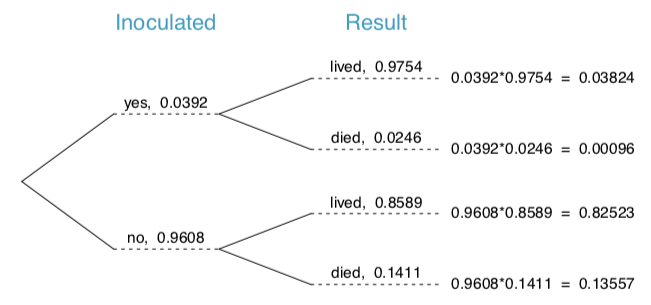
\includegraphics[scale=0.5]{images/tree.png}
    \end{center}
\end{frame}

\begin{frame}{Tree Diagrams}
    \begin{center}
        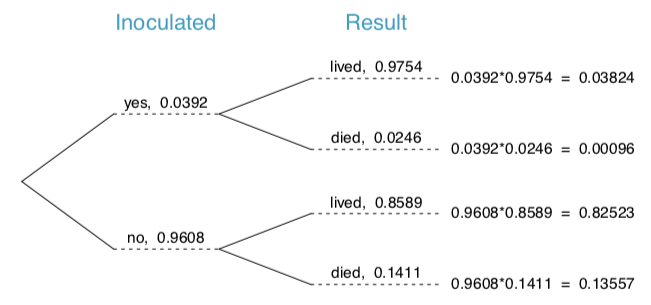
\includegraphics[scale=0.3]{images/tree.png}
    \end{center}
    \begin{itemize}
        \item The first branch, for \texttt{inoculation}, is called the \textbf{primary branch}.
        \item All other branches, in this case for \texttt{result} are \textbf{secondary branches}.
    \end{itemize}
\end{frame}

\begin{frame}{Tree Diagrams}
    \begin{center}
        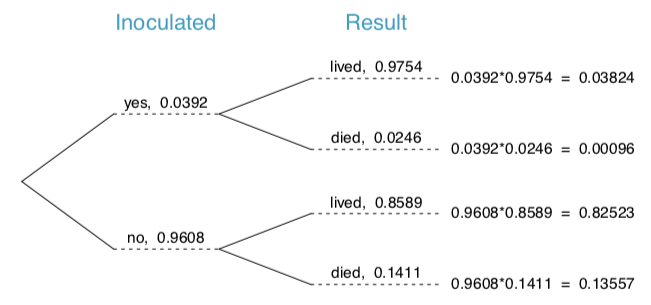
\includegraphics[scale=0.3]{images/tree.png}
    \end{center}
    \begin{itemize}
        \item The probabilities for the primary branch are marginal.
        \begin{itemize}
            \item For \texttt{inoculation} is \texttt{yes}, the marginal probability is $P(\texttt{inoculation} \text{ is } \texttt{yes})=0.0392$.
        \end{itemize}
        \item The probabilities for the secondary branches are conditional.
        \begin{itemize}
            \item For \texttt{result} is \texttt{lived} on the \texttt{inoculation} is \texttt{yes} branch, we have $P(\texttt{result} \text{ is } \texttt{lived } |\texttt{ inoculation} \text{ is } \texttt{yes})=0.9754$
        \end{itemize}
    \end{itemize}
\end{frame}

\begin{frame}{Tree Diagrams}
    \begin{center}
        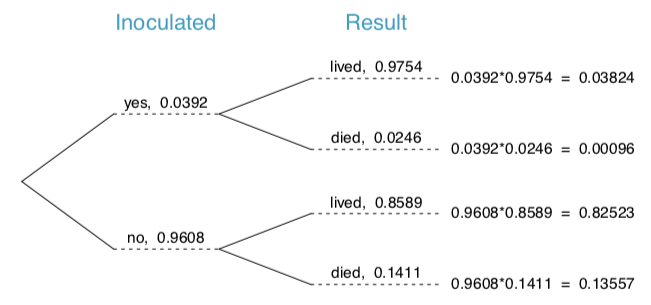
\includegraphics[scale=0.3]{images/tree.png}
    \end{center}
    \begin{itemize}
        \item Joint probabilities are shown to the right of each secondary branch.
        \item These are computed using the General Multiplication Rule
        \[
        P(A\text{ and }B)=P(A|B)\times P(B)
        \]
        where the primary branch represents event $B$ and the secondary branch event $A$.
    \end{itemize}
\end{frame}

\begin{frame}{Example: Exam Scores}
    Consider the midterm and final for a statistics class. 
    \begin{itemize}
        \item Suppose 13\% of students earned an A on the midterm. 
        \item Of those students who earned an A on the midterm, 47\% received an A on the final.
        \item 11\% of the students who earned lower than an A on the midterm received an A on the final.
        \item You pick up a final exam at random and notice the student received an A.
    \end{itemize} 
    What is the probability that this student earned an A on the midterm?
\end{frame}

\begin{frame}{Example: Exam Scores}
    Let's start by writing the given information in probability notation.
    \begin{itemize}
        \item $P(\texttt{midterm}=\texttt{A})=0.13$
        \item $P(\texttt{final}=\texttt{A } | \texttt{ midterm}=\texttt{A})=0.47$
        \item $P(\texttt{final}=\texttt{A } | \texttt{ midterm}=\texttt{not A})=0.11$
    \end{itemize}
    \vspace{12pt}We want to know the probability that a student who earned an A on the final also earned an A on the midterm:
    \[
    P(\texttt{midterm}=\texttt{A }|\texttt{ final}=\texttt{A})
    \]
\end{frame}

\begin{frame}{Example: Exam Scores}
    Now that we've formalized the information from the problem statement, we can consider our next steps.
    
    \vspace{12pt}It's not yet clear how to calculate 
    \[P(\texttt{midterm}=\texttt{A }|\texttt{ final}=\texttt{A}),\]
    so let's use what we know to draw a tree diagram.
\end{frame}

\begin{frame}{Example: Exam Scores}
    We will use this information to draw our tree diagram.
    \begin{itemize}
        \item $P(\texttt{midterm}=\texttt{A})=0.13$
        \item $P(\texttt{final}=\texttt{A } | \texttt{ midterm}=\texttt{A})=0.47$
        \item $P(\texttt{final}=\texttt{A } | \texttt{ midterm}=\texttt{not A})=0.11$
    \end{itemize}
\end{frame}

\begin{frame}{Example: Exam Scores}
    \begin{center}
        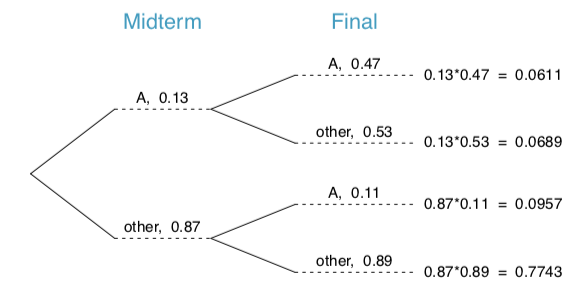
\includegraphics[scale=0.5]{images/tree2.png}
    \end{center}
    Can we use this to calculate $P(\texttt{midterm}=\texttt{A }|\texttt{ final}=\texttt{A})$?
\end{frame}

\begin{frame}{Example: Exam Scores}
    First, consider our conditional probability formula.
    \[
        P(\texttt{midterm}=\texttt{A }|\texttt{ final}=\texttt{A}) = \frac{P(\texttt{midterm}=\texttt{A }\text{and}\texttt{ final}=\texttt{A})}{P(\texttt{final}=\texttt{A})}
    \]
    We can get all of the probabilities on the right hand side of the formula by using our tree diagram!
\end{frame}

\begin{frame}{Example: Exam Scores}
    \begin{center}
        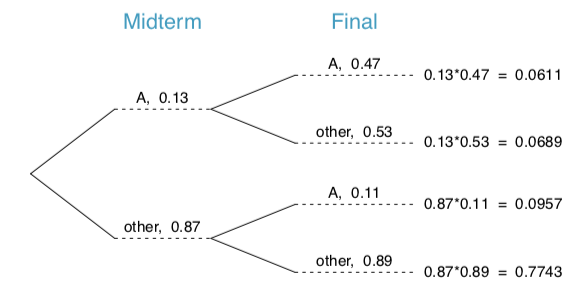
\includegraphics[scale=0.4]{images/tree2.png}
    \end{center}
    First,
    \[
    P(\texttt{midterm}=\texttt{A }\text{and}\texttt{ final}=\texttt{A})=0.0611.
    \]
\end{frame}

\begin{frame}{Example: Exam Scores}
    \begin{center}
        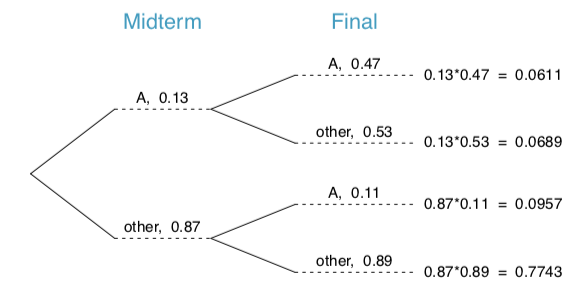
\includegraphics[scale=0.4]{images/tree2.png}
    \end{center}
    Then
    \small\begin{align*}
        P(&\texttt{final}=\texttt{A}) \\
        &=P(\texttt{midterm}=\texttt{not A}\text{ and }\texttt{final}=\texttt{A}) +P(\texttt{midterm}=\texttt{A}\text{ and }\texttt{final}=\texttt{A}) \\
        &= 0.0957 + 0.0611 =0.1568
    \end{align*}
\end{frame}

\begin{frame}{Example: Exam Scores}
    Plugging these in,
    \begin{align*}
        P(\texttt{midterm}=\texttt{A }|\texttt{ final}=\texttt{A}) &= \frac{P(\texttt{midterm}=\texttt{A }\text{and}\texttt{ final}=\texttt{A})}{P(\texttt{ final}=\texttt{A})} \\
        &= \frac{0.0611}{0.1568} = 0.3897.
    \end{align*}
    
    \vspace{12pt}So the probability that a student earned an A on the midterm, given that their final exam score was an A, is about 39\%.
\end{frame}

\begin{frame}{Bayes' Theorem}
    That was a lot of work! 
    
    \vspace{12pt} Bayes' Theorem will help minimize this work so that we can more easily calculate
    \[
        P(\text{statement about variable 1 }|\text{ statement about variable 2})
    \]
    when we have information about
    \[
        P(\text{statement about variable 2 }|\text{ statement about variable 1}).
    \]
\end{frame}

\begin{frame}{Bayes' Theorem}
    \vspace{12pt} Bayes' Theorem will help us more easily calculate
    \[
        P(\text{statement about variable 1 }|\text{ statement about variable 2})
    \]
    when we have information about
    \[
        P(\text{statement about variable 2 }|\text{ statement about variable 1}).
    \]
\end{frame}

\begin{frame}{Example: Mammograms}
    \begin{itemize}
        \item About 0.35\% of women over 40 will develop breast cancer in any given year.
        \item In about 11\% of patients with breast cancer, a mammogram test gives a \textbf{false negative}.
        \begin{itemize}
            \item This means that the test indicates \textit{no cancer} even though cancer is present.
        \end{itemize}
        \item In about 7\% of patients without breast cancer, the test gives a \textbf{false positive}.
        \begin{itemize}
            \item This is when the test says that there \textit{is cancer} when actually there is not.
        \end{itemize}
    \end{itemize}
\end{frame}

\begin{frame}{Example: Mammograms}
    If we tested a random woman over 40 for breast cancer using a mammogram and the test came back positive for cancer, what is the probability that the patient actually has breast cancer?
\end{frame}

\begin{frame}{Example: Mammograms}
    \begin{itemize}
        \item We know that 11\% of the time, a mammogram gives a false negative.
        \item We can use the complement to find the probability of testing positive for a woman with breast cancer:
        \[
        1-0.11=0.89
        \]
        \item But we want the probability of cancer given a positive test result.
    \end{itemize}
\end{frame}

\begin{frame}{Example: Mammograms}
    We can break this probability down into its component parts
    \[
        P(\text{BC } | \text{ mammogram+}) = \frac{P(\text{BC and mammogram+})}{P(\text{ mammogram+})}
    \]
    where BC denotes breast cancer and mammogram+ denotes a positive breast cancer screening.
\end{frame}

\begin{frame}{Example: Mammograms}
    We can construct a tree diagram from these probabilities:
    \begin{center}
        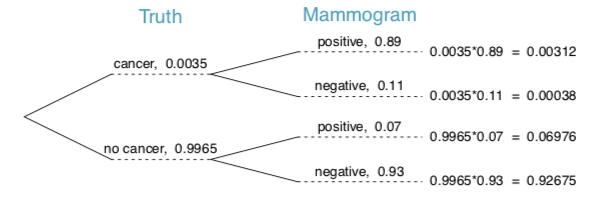
\includegraphics[scale=0.55]{images/treemam.png}
    \end{center}
\end{frame}

\begin{frame}{Example: Mammograms}
    Returning to our desired probability,
    \[
        P(\text{BC } | \text{ mammogram+}) = \frac{P(\text{BC and mammogram+})}{P(\text{ mammogram+})},
    \]
    the probability that a patient has cancer and the mammogram is positive is
    \begin{align*}
    P(\text{BC and mammogram+}) &= P(\text{mammogram+ } | \text{ BC})\times P(\text{has BC}) \\
    &= 0.89 \times 0.0035 = 0.00312
    \end{align*}
\end{frame}

\begin{frame}{Example: Mammograms}
    The probability that the mammogram is positive is
    \small\begin{align*}
        P(&\text{mammogram+}) \\ 
        &=P(\text{mammogram+ and BC}) + P(\text{mammogram+ and no BC}) \\
        &= P(BC)P(\text{mammogram+ }|\text{ BC}) + P(\text{no BC})P(\text{mammogram+ }|\text{ no BC}) \\
        &= 0.0035 \times 0.89 + 0.9965 \times 0.07 = 0.07288
    \end{align*}
\end{frame}

\begin{frame}{Example: Mammograms}
    Plugging these back in,
    \begin{align*}
        P(\text{BC } | \text{ mammogram+}) &= \frac{P(\text{BC and mammogram+})}{P(\text{ mammogram+})} \\
        &= \frac{0.00312}{0.07288} = 0.0428
    \end{align*}
    Even if a patient has a positive mammogram screening, there is still only a 4\% chance of breast cancer!
    
    \vspace{12pt}This is why doctors usually run several tests before deciding that a person has a (relatively) rare disease or condition.
\end{frame}

\begin{frame}{Law of Total Probability}
    Notice that the denominator of the previous equation was
    \begin{small}\begin{align*}
        P(&\text{mammogram+ and BC}) + P(\text{mammogram+ and no BC}) \\
        &= P(BC)P(\text{mammogram+ }|\text{ BC}) + P(\text{no BC})P(\text{mammogram+ }|\text{ no BC})
    \end{align*}\end{small}
    This is the sum of the probabilities for each positive screening scenario.
\end{frame}

\begin{frame}{Law of Total Probability}
    For two events $A$ and $B$, the Law of Total Probability states
    \[
    P(B) = P(B|A_1)P(A_1)+P(B|A_2)P(A_2)+\dots +P(B|A_k)P(A_k)
    \]
    where $A_1 \dots A_k$ are the $k$ possible outcomes for event $A$.
\end{frame}

\begin{frame}{Bayes' Theorem}
    Consider the following conditional probability for variable 1 and variable 2: 
    \[
    P(\text{outcome }A_1\text{ of variable 1 }|\text{ outcome }B\text{ of variable 2})
    \]
    
    Bayes’ Theorem states that this conditional probability can be identified as the following fraction
    \[
        \frac{P(B|A_1)P(A_1)}{P(B|A_1)P(A_1)+P(B|A_2)P(A_2)+\dots +P(B|A_k)P(A_k)}
    \]
\end{frame}

\begin{frame}{Bayes' Theorem}
    Bayes' Theorem is a generalization of what we've been doing with tree diagrams. 
    \begin{itemize}
        \item The numerator identifies the probability of getting both $A_1$ and $B$. 
        \item The denominator is the marginal probability of getting $B$. 
        \item This bottom component of the fraction looks complicated since we have to add up probabilities from all of the different ways to get $B$. 
    \end{itemize}
\end{frame}

\begin{frame}{Bayes' Theorem}
    To apply Bayes’ Theorem correctly, there are two preparatory steps:
    \begin{enumerate}
        \item Identify the marginal probabilities of each possible outcome of the first variable.
        \[
            P(A_1), P(A_2), \dots, P(A_k)
        \]
        \item Identify the probability of the outcome $B$, conditioned on each possible scenario for the first variable.
        \[
            P(B|A_1), P(B|A_2), \dots, P(B|A_k)
        \]
    \end{enumerate}
    When each of these has been identified, they can be plugged into Bayes' Theorem.
\end{frame}

\begin{frame}{Bayes' Theorem}
     Bayes’ Theorem tends to be a good option when there are so many scenarios that drawing a tree diagram would be very complex.
     
     \vspace{12pt}Each probability is found and identified in the same way as when creating a tree diagram.
     
     \vspace{12pt}Unless specifically asked to use either a tree diagram or Bayes' Theorem, you may use whichever method you prefer.
\end{frame}

\begin{frame}{Monty Hall Problem}
    The Monty Hall problem comes from an old game show. There are three doors. Behind one of the doors is a car. Behind the other two doors there are goats. The goal is to win the car.
\end{frame}

\begin{frame}{Monty Hall Problem}
    \begin{center}
        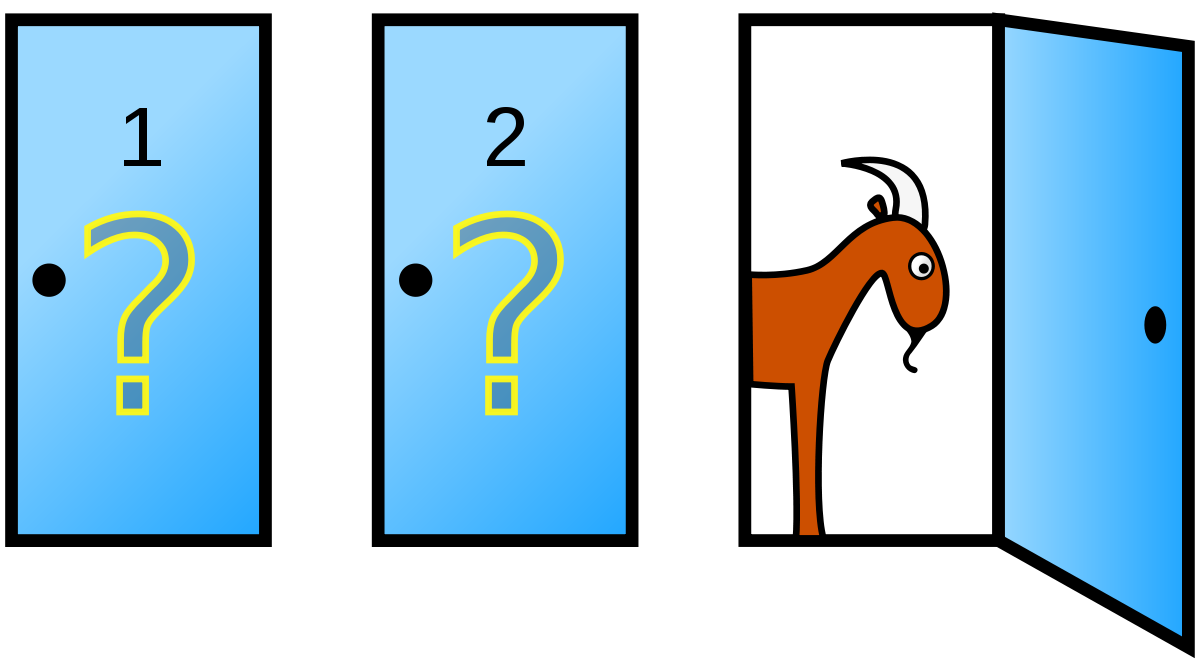
\includegraphics[scale=0.2]{images/montyhall.png}
    \end{center}
    You begin by choosing a door. The host then opens one of the other two doors, always such that the opened door reveals a goat.
\end{frame}

\begin{frame}{Monty Hall Problem}
    You then have the option to stay with your original choice or switch to the remaining unopened door.
    
    \vspace{12pt}Would you switch or stay? Does it matter?
\end{frame}

\begin{frame}{Monty Hall Problem}
    Intuition suggests that there is a 50\% chance of each of the remaining doors contain the car.
    
    \vspace{12pt}We will examine this using (1) a visual and (2) Bayes' Theorem.
\end{frame}

\begin{frame}{Monty Hall Problem: Visual}
    The order of the doors doesn't matter, so for convenience we suppose that we start by choosing Door 1. The host always shows us a door with no goat. Let's see what happens in each scenario:
    
    \begin{center}
        \begin{tabular}{ccc cc}
            Door 1 & Door 2 & Door 3 & Stay & Switch \\
            \hline
            Goat & Goat & \textbf{Car} & Lose & \textbf{Win} \\
            Goat & \textbf{Car} & Goat & Lose & \textbf{Win} \\
            \textbf{Car} & Goat & Goat & \textbf{Win} & Lose
        \end{tabular}
    \end{center}
    2/3 of the time, switching leads to a win!
\end{frame}

\begin{frame}{}
    \begin{center}
        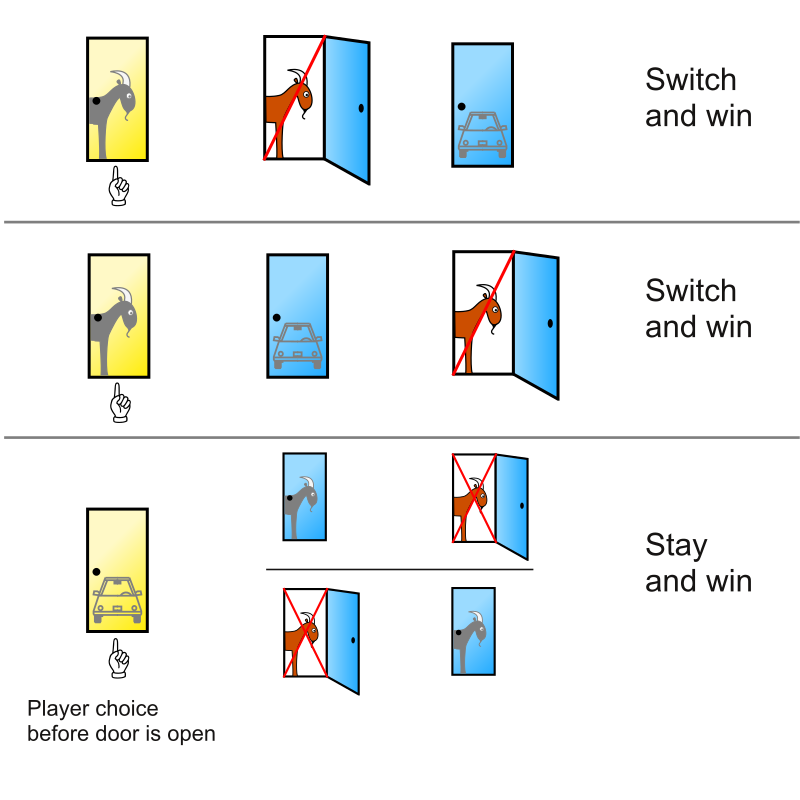
\includegraphics[scale=0.3]{images/montyhall2.png}
    \end{center}
\end{frame}

\begin{frame}{Monty Hall Problem: Bayes' Theorem}
    Let $D_A$ be the event that Door A has a car behind it, $D_B$ the event that Door B has a car behind it, and $D_C$ the event that Door C has a car behind it. Let $H_B$ be the event that the host opens Door B. 
\end{frame}

\begin{frame}{Monty Hall Problem: Bayes' Theorem}
    Suppose we choose Door A. We want to know
    \[
        P(D_A | H_B) = \frac{P(D_A \text{ and }H_B)}{P(H_B)}
    \]
    or the probability that the car is behind Door A, our original choice, given that the host opened Door B. This is the probability that we \textbf{win} when we \textbf{stay}.
\end{frame}

\begin{frame}{Monty Hall Problem: Bayes' Theorem}
    First,
    \begin{align*}
        P(D_A \text{ and }H_B) &= P(H_B | D_A)P(D_A) \\
        &= \frac{1}{2}\times\frac{1}{3} \\
        &= \frac{1}{6}
    \end{align*}
    \vspace{12pt}Why does $P(H_B | D_A)=1/2$?
\end{frame}

\begin{frame}{Monty Hall Problem: Bayes' Theorem}
    Then we need to find $P(H_B)$. Using the Law of Total Probability,
    \begin{align*}
        P(H_B) &= P(H_B|D_A)P(D_A)+P(H_B|D_B)P(D_B)+P(H_B|D_C)P(D_C) \\
        &= \frac{1}{2}\times\frac{1}{3} + 0\times\frac{1}{3} + 1\times\frac{1}{3} \\
        &= \frac{1}{6} + 0 + \frac{1}{3} \\
        &= \frac{1}{2}
    \end{align*}
\end{frame}

\begin{frame}{Monty Hall Problem: Bayes' Theorem}
    Plugging these back into our equation for Bayes' Theorem,
    \begin{align*}
        P(D_A | H_B) &= \frac{P(D_A \text{ and }H_B)}{P(H_B)} \\
        &= \frac{1}{6}\bigg/\frac{1}{2} \\
        &= \frac{1}{3}
    \end{align*}
    So the probability of winning if we stay with our original door is 1/3! 
\end{frame}